
\documentclass[a4paper]{article}
%\usepackage{lua-visual-debug}
\usepackage[utf8]{inputenc}
\usepackage{amsmath,amssymb,amsfonts}
\usepackage{graphicx}
\usepackage{hyperref}
\usepackage{wrapfig}
\usepackage{subcaption}
\usepackage{parskip}
\usepackage{url}
\usepackage{graphicx}
\usepackage{float}
\usepackage[numbers]{natbib}
\usepackage{natbib}
\usepackage[margin=2.5cm]{geometry}
\usepackage[title]{appendix}
\usepackage{tikz}
\usepackage{siunitx} %\SI{1500}{kg^2}, %\si{kg^2}
\usetikzlibrary{calc}
\bibliographystyle{unsrt}
\usepackage{enumitem}
\usepackage{bm}
\usepackage{pdfpages}
\usepackage{mathtools}

\DeclarePairedDelimiter{\ceil}{\lceil}{\rceil}

\title{ID2209 - Distributed Artificial Intelligence and Intelligent Agents Assignment 1 - Festival Simulation}
\author{Kishore Kumar, kishorek@kth.se \and Abel Valko, valko@kth.se}
\date{November 2021}

\setlength{\parindent}{0pt}

\begin{document}

\maketitle

\section{Introduction}
The objective of this assignment was to model a festival with 3 types of agents namely, Guest, Store and Information Center (and a fourth one called as Security, added as part of Challenge 2). The 'Guest' agents attend the festival and wander around aimlessly. They get hungry or thirsty based on certain probabilities, at which point they will want to go to an information desk to ask for directions to the food/drink Stores. Once they get the directions, they go to the respective stores to fulfill their thirst/hunger and they return to "dancing". 

\subsection{How To Run}
Open Gama and import the models found in folder "Lab 1". The experiments can be run by clicking the FestivalExperiment button. The model can be tweaked using the following parameters:
\begin{itemize}
    \item \textit{numberOfGuests}, \textit{numberOfStoresFood}, \textit{numberOfStoresDrink}, and \textit{numberOfInfoCenters} control the number of created agents of each type
    \item \textit{hungerProb} and \textit{thirstProb} determine the probability of a guest becoming hungry or thirsty at each timestep
    \item The visual representation of each agent can be altered by changing the base aspect. Colour, shape and size can be set here.
\end{itemize}

\section{Species}

\subsection{Guest}
The guest agents represent the visitors to the festival. They get hungry and thirsty with certain probabilities (set by variables as stated above), move to the closest information center to ask for directions to the nearest store with food/drink, move to the store and once no longer hungry or thirsty keep dancing (wandering). Their hunger and thirst state is kept track of through the \textit{hungry} and \textit{thirsty} variables while their eventual objectives are stored in the \textit{foodObjective}, \textit{drinkObjective}, and \textit{infoObjective} variables. The guest agent is shown as a circle of different possible colours dependent on its state. It is green when it is neither hungry nor thirsty, blue when it is only thirsty, red when it is only hungry, and purple when it is both hungry and thirsty.
The Guest agents have four reflexes and one action, as well as the moving skill. The reflexes are:
\begin{itemize}
    \item \textit{updateHungerAndThirst} which updates the hunger and thirst state with probabilities set as mentioned above.
    \item \textit{move} which makes the agent move towards its objective if this is set in the \textit{objective} variables as mentioned above. The objective priority order is $drink > food > info$. However, if the agent is already on its way to the food store eat when getting thirsty it will complete that objective before moving on to finding a store with drinks. If no objective is set, i.e. the guest is neither hungry nor thirsty, it wanders. Default parameters from the moving skill are used.
    \item \textit{checkForInfo} triggers if the guest is hungry or thirsty and has arrived at (is close to) an info center. The guest then asks the info center for directions to the nearest place that fulfills its hunger/thirst.
    \item \textit{consumeStuff} triggers if the guest is near a store. If the guest is hungry it will "eat" and reset its \textit{hunger} and \textit{foodObjective}. The same is done for thirst. 
\end{itemize}
The Guests only action is \textit{updateInfoObjective}. This is done when the guest becomes thirsty (see \textit{updateHungerAndThirst}). It is assumed that the guest always knows where the nearest information center is (or that there are simply clear signs at the festival) and goes to the nearest one when they get hungry or thirsty. It is further assumed that the guest has no memory, and so will not remember the location of any stores in the future. While in practice the guest may steer off course in order to go to a store they see nearby, even if they have not received directions to it yet from the information center, the model assumes that the guest is "blind" and only follows the precise instruction given to it.

\subsection{InformationCenter}
The \textit{InformationCenter}s are stationary agents which have information on the exact location of the closest stores with food and drink, these are stored in the \textit{closestFood} and \textit{closestDrink} variables respectively. They are visually represented as black squares. The only action they possess is the \textit{setClosestStores} action which, being similar to the \textit{Guest}'s \textit{updateInfoObjective}, sets the closest stores. This could also be implemented using an initialization function, since the information centers and stores are stationary.

\subsection{Store}
The \textit{Store}s are also stationary agents which serve either food or drink. We can define a store as either a food or drink store by using the attribute \textit{type} of the \textit{Store} agents. The \textit{Store} agents are visually represented as triangles whose colour depends on whether the store is a food store or a drink store. The food stores are red in colour while the drink stores are blue in colour. The stores are implemented inside the initialisation function by specifying the number of food stores and the number of drink stores. The Store agents do not have any reflexes or actions, thus rendering them incapable of performing any intelligent functions like the guests or the information centers.  

\section{Implementation}
First all agents were created without any actions or reflexes. The \textit{updateHungerAndThirst} reflex was then added to the \textit{Guest}s. The guests were then given the \textit{updateInfoObjective} and the \textit{move} reflex such that they would turn hungry or thirsty, update their nearest information center, and move to it. The \textit{Store}s were then split into containing food or drink, using their \textit{type} variable. The \textit{InformationCenter}s were given the \textit{setClosestStores} action, so that they have the location of the closest stores saved and the \textit{Guest}s were given the \textit{checkForInfo} reflex. Finally, the \textit{Guest}s were edited to move to their food/drink objective and were given the \textit{consumeStuff} reflex, thereby completing the task.

\section{Results}
As can be seen from Figure \ref{fig:printout} the task was successfully completed. In this printout the actions of one \textit{Guest} can be seen. The following events occur:
\begin{enumerate}
    \item The \textit{Guest} begins off not hungry nor thirsty and is simply wandering at the festival.
    \item The \textit{Guest} then gets thirsty and goes to the nearest information center.
    \item The \textit{Guest} receives the location of the nearest store with drinks
    \item While on their way to the store the \textit{Guest} gets hungry, but continues to the store with drinks and quenches their thirst.
    \item After drinking, the \textit{Guest} will move again towards the information center to ask for directions for food. During this time they become thirsty again.
    \item The \textit{Guest} arrives at the information center and receives directions to both food and drink.
    \item The \textit{Guest} prioritizes drinking, and so moves to the store with drinks first and then to the store with food.
    \item The \textit{Guest} is then satisfied and returns to "dancing", i.e. wandering.
\end{enumerate}

\begin{figure}[H]
    \centering
    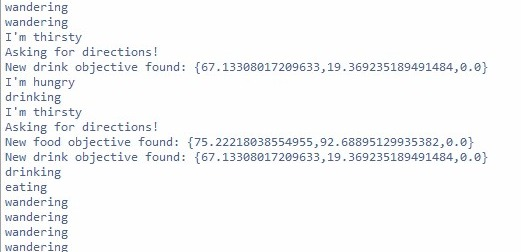
\includegraphics[scale=0.5]{printout.jpeg}
    \caption{Command line printout for simulation with one \textit{Guest} agent}
    \label{fig:printout}
\end{figure}

A screenshot of this can be seen in Figure \ref{fig:1agent} where the green circle represents the \textit{Guest}, which is wandering around as it is neither hungry nor thirsty. The blue triangles the \textit{Store}s with drink, the red triangles the \textit{store}s with food, and the black squares the \textit{InformationCenter}s.

\begin{figure}[H]
    \centering
    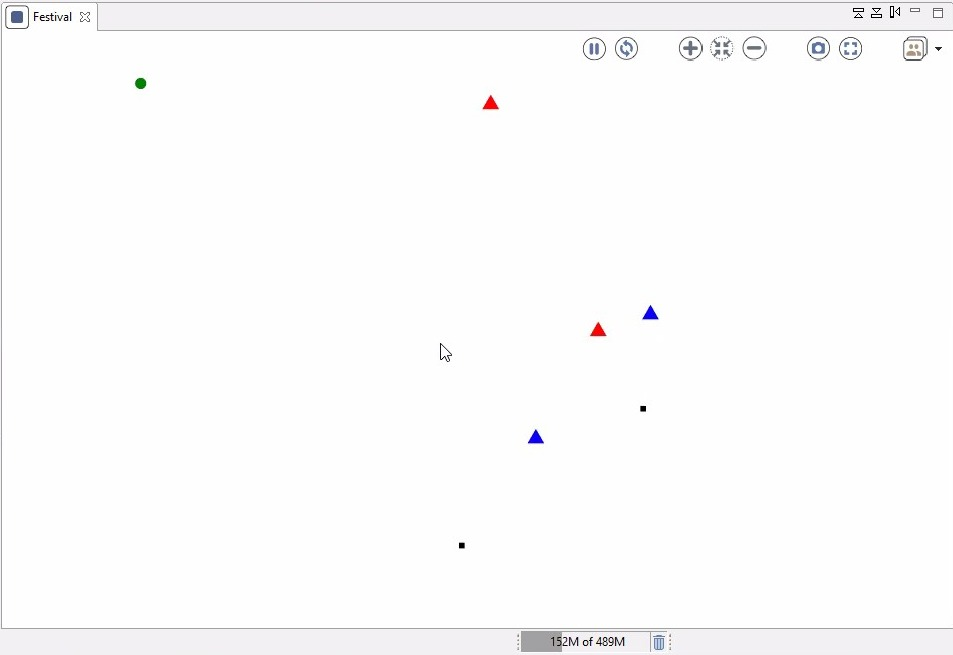
\includegraphics[scale=0.3]{1agent.jpeg}
    \caption{Screenshot from simulation graphics for one \textit{Guest} agent}
    \label{fig:1agent}
\end{figure}

No printout is show for the case with many \textit{Guest}s for simplicity's sake, but a screenshot can be seen in Figure \ref{fig:manyagent}.

\begin{figure}[H]
    \centering
    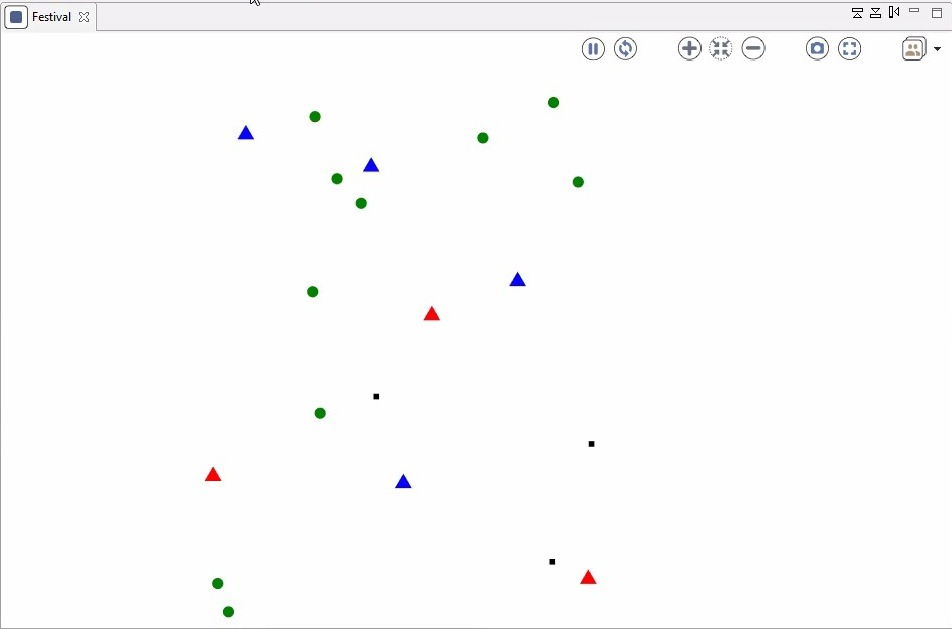
\includegraphics[scale=0.3]{manyagent.jpeg}
    \caption{Screenshot from simulation graphics for 10 \textit{Guest} agents}
    \label{fig:manyagent}
\end{figure}

\section{Challenge 1}
The objective of challenge 1 was to implement some memory of previous places in the \textit{Guest}s and let them go to a new place with certain probability. This was done by adding variables which save the locations of the previous stores visited, these are \textit{rememberFood} and \textit{rememberDrink}. The \textit{Guest} then has a certain probability of going back to the remembered location next time they are hungry or thirsty. Otherwise they visit the nearest \textit{InformationCenter} and ask for directions. The store that the InformationCenter suggests will also be random, and not necessarily the closest store. This results in the \textit{Guest} visiting multiple different stores, as well as not always returning to the \textit{InformationCenter} to ask for directions.

The distance travelled depends strongly on the various parameters. The likelihood with which the \textit{Guest} uses their remembered \textit{Store}, the number of \textit{Store}s, the spread of the \textit{Store}s, as well as the number and location of \textit{InformationCenter}s all influence the distance travelled. In certain cases this may be lower than for the base case (implementation above) while for others it may be more. In particular, the larger the probability of using remembered values and the smaller the spread of \textit{InformationCenter}s and \textit{Stores} the less distance the \textit{Guest} travels. Conversely, the larger the spread of stores and lower the likelihood of using stored values the more distance the \textit{Guest} will travel. This behaviour is to be expected. With larger probability of remembering the \textit{Guest} has a larger chance of going directly to a store and not via an \textit{InformationCenter}. The random recommendation of \textit{Stores} however increases the distance travelled, as there is a chance that non-optimal locations are suggested.

\section{Challenge 2}
The challenge 2 is built on top of the challenge 1 implementation, where there are \textit{Guest}s, \textit{InformationCenter}s and \textit{Store}s. The \textit{Guest}s go to \textit{InformationCenter}s if they are hungry and remember the location of the food and drink stores. The agent can go back to the \textit{Store}s or the \textit{InformationCenter}s depending on a probability manually set by the user. The following changes/additions have been made to implement challenge 2:
\begin{enumerate}
    \item The \textit{Guest} agents have an additional attribute \textit{good}, which decides if the \textit{Guest} agent is good or bad. This is randomly assigned to the agents using a \textit{flip} function with a 50 percent probability of being good or bad.
    \item The good agents have the original colour scheme while the bad agents are black in colour if they are neither hungry or thirsty, pink in colour if they are both hungry and thirsty, maroon in colour if they are hungry and not thirsty and yellow in colour if they are thirsty and not hungry.
    \item The bad \textit{Guest} agents do the exact same functions performed by the good \textit{Guest} agents (Get hungry/thirsty ,go to information center to get the shop locations and fulfill the hunger/thirst by going to the shops).
    \item There is a new species called as \textit{Security} which represents the cop. These agents are tasked with going to the information center if called, retrieve the bad guest information from the information centers and kill the bad guests if within proximity.
    \item The \textit{Security} agents are grey in colour and are represented by large circles.
    \item The \textit{Security} agents have an action to set their name, a reflex called as \textit{getBadGuyName} that kicks in if the security is close to an information center and a \textit{move} reflex which causes the agent to wander, move towards an Information Center or chase a bad guest depending on its state.
    \item The \textit{InformationCenter} agents have a new internal variable of the type string called as \textit{badGuyName}, which stores the name of the bad \textit{Guest} agent.
    \item To store the name of the bad agent as mentioned above, the \textit{InformationCenter} has a new reflex implemented on it called as \textit{reportBadGuy}, which is activated when there is a \textit{Guest} agent very close to it. The \textit{InformationCenter} agent checks if the guest agent's type is good or bad. If the agent is bad, the \textit{InformationCenter} stores the name of the bad agent and calls one of the available cops(\textit{Security} agents) by giving that \textit{Security} agent an \textit{infoObjective}. 
    \item The cop now moves towards the information center that called it and receives the \textit{badGuyName} through the \textit{getBadGuyName} reflex.
    \item The cop compares the name it received with the names of all the \textit{Guest} agents alive and finds the bad agent that visited the information center. It sets the bad agent as its target and goes towards it. All these actions take place in the \textit{move} reflex of the \textit{Security} agent.
    \item The \textit{Guest} agents have a new reflex called as \textit{agent\_die}, which is kicked in if the agent is near a cop and the agent is bad. This reflex decreases the \textit{numberOfGuests}, resets the state of the cop close to it and finally kills the bad agent using the \textit{die} function.
\end{enumerate}

\begin{figure}[H]
    \centering
    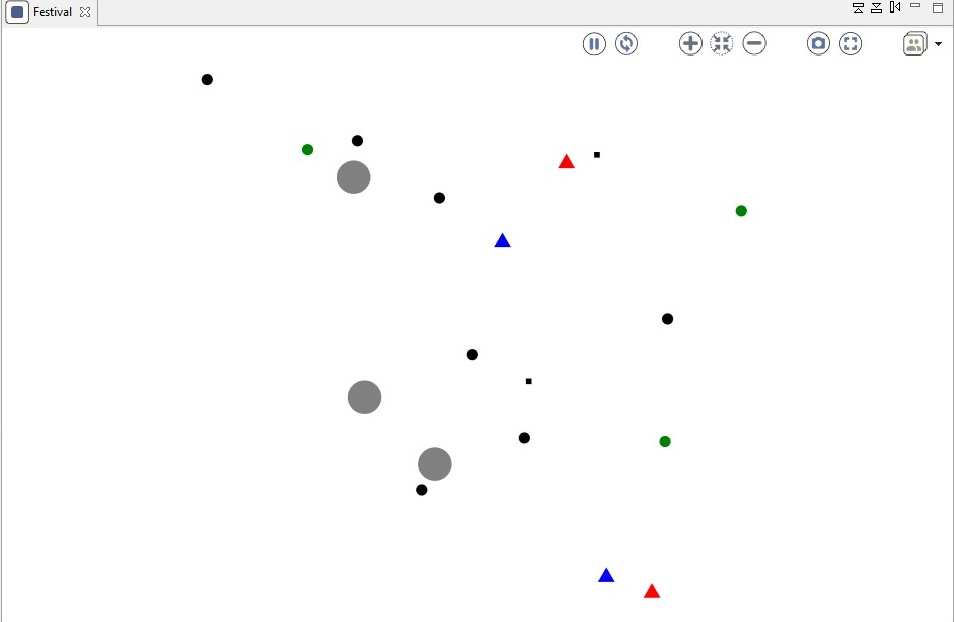
\includegraphics[scale=0.5]{cop_sim.jpg}
    \caption{Screenshot from simulation graphics for multiple "security guards" and "bad guys"}
    \label{fig:cop_sim}
\end{figure}

\begin{figure}[H]
    \centering
    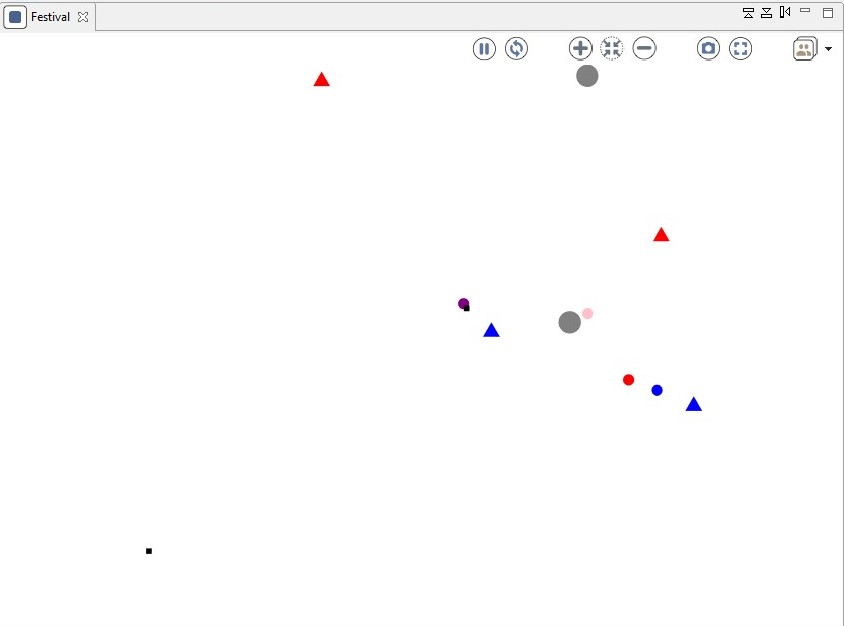
\includegraphics[scale=0.5]{cop chase.jpg}
    \caption{Screenshot from simulation graphics for "security guard" chasing "bad guy"} 
    \label{fig:cop_chase}
\end{figure}

\begin{figure}[H]
    \centering
    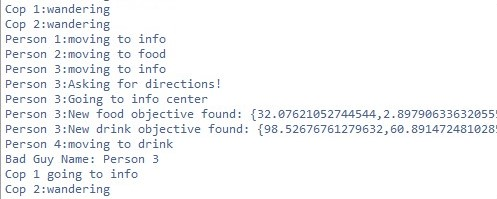
\includegraphics[scale=0.7]{bad guy info center console.jpg}
    \caption{Console readout for bad guy being recognized at information center}
    \label{fig:bad_guy_info}
\end{figure}

\begin{figure}[H]
    \centering
    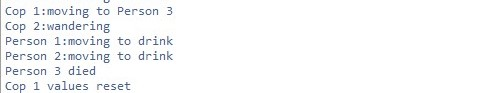
\includegraphics[scale=0.7]{cop kills.jpg}
    \caption{Console readout for cop chasing and killing bad guy}
    \label{fig:cop_kills}
\end{figure}

While running the simulation, the cops will wander around and eventually proceed to the information centers and kill the bad guests while leaving the good guests.

\section{Discussion}
Implementing the base case was straight forward. However, some nuances are lost in such a modelling. We considered, but did not implement, a number of behaviours which would make edge cases behave more realistically. For example, \textit{Guest}s would likely be able to see and go to stores which are nearby when on the way to \textit{InformationCenters}. It is also worth noting that the probability distribution used for hunger and thirst is rather unrealistic. A fixed probability of getting hungry or thirsty in each timestep is used, while in practice this distribution may be better modelled as Poisson.

Some of the implementation may also be non-optimal considering the Gama modelling language was new to the group. However, we gained some insights into what modelling decisions are less or more ideal when considering future work and what structures may be scalable and readable in the future. 

The implementation of Challenge 1 was done quite simply, as no detailed instructions were given, but it demonstrated well how a model can be built upon and modified. It also highlighted some aspects of the modelling process which aid or hinder future work. We also noted that communication can often be done in multiple ways and even initiated by both parties. This means that decisions on how communication should be modelled (such as who should possess the relevant reflex) are critical. In certain cases the implementation which is simplest in code for example may not be the one which models the actions best in real life.

Challenge 2 was implemented according to the instructions, though a different interpretation (clarified later, but not soon enough for a new implementation to be made) may be more realistic. Here again the conclusion may be drawn that the logic of the model can be implemented in multiple ways and should be selected based on the purpose. The "realistic" implementation may not always be the best. This may be unnecessarily complicated, lead to unscalable or even unreadable solutions. Overall, the objective of the model should motivate the implementation.

While the modelling was interesting in and of itself we wished there would be more opportunities for drawing conclusions from the simulation, particularly of a nature which can influence policy or strategy in some way. For example, how would one draw numerical conclusions from such a simulation? How could the simulation results be analyzed?

\end{document}

